\clearpage
\begin{figure}[H]
    \centering
    \begin{adjustbox}{width=12cm,center}
    \frame{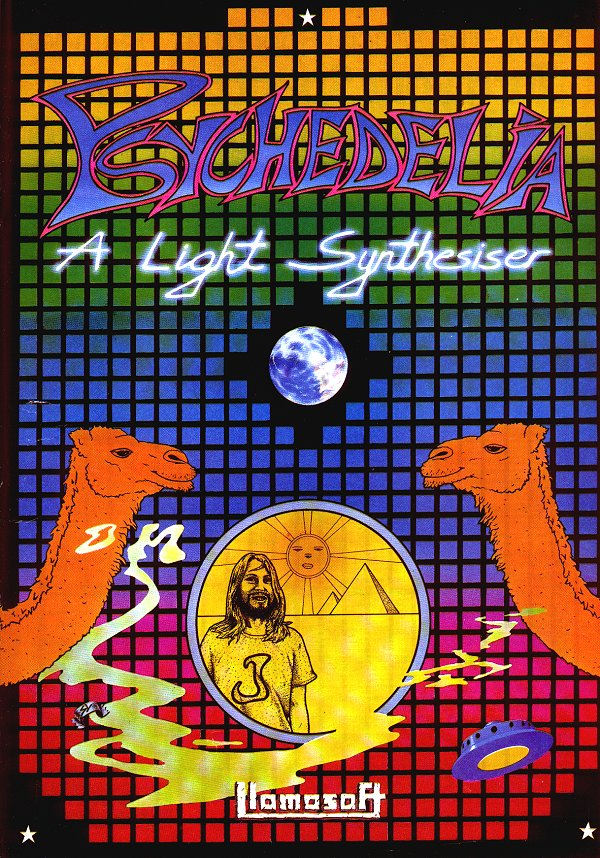
\includegraphics{src/preface/psychedelia.jpg}}%
    \end{adjustbox}
\caption{Cover art by Steinar Lund for the commercial edition of Psychedelia}
\end{figure}
\clearpage
\chapter*{About This Book} 
This is a book about a toy. A toy that was the first of its kind. A kind of toy that has never really caught on,
though maybe its moment lies some way in the future. 

We are going to take apart the toy to see how it works. THe pieces are all over the floor and they seem to be made
of strange-looking computer instructions, I hope we know what we're doing...


\section*{Note on the Text}
The version you are reading is little more than a scrapbook still many revisions away from a
finished product. If you find the writing hard going or the attempts to explain things difficult
to follow, by all means \href{https://github.com/mwenge/psypixels/issues}{\textcolor{blue}{leave me a note}} and
I will gratefully accept your complaint. In the meantime, please skip over any blemishes
to the next pretty picture or promising-looking block of text.

The full source code is available in \href{https://github.com/mwenge/psychedelia}{\textcolor{blue}{its own Github repository}}. 
You should find that it matches exactly the snippets of code provided in the book, though in some cases the extracts in the book have been edited
and reformatted for brevity.


Rob Hogan (\href{https://mastodon.social/@mwenge}{\textcolor{blue}{@mwenge}})\\
Dublin \the\year{} \\

\clearpage
\clearpage
\shipout\null
\vspace*{\fill}
\begin{figure}[H]
    \centering
      
\includegraphics[width=5cm]{src/cover/title_page.png}%
\end{figure}
\vspace*{\fill}
\thispagestyle{empty}%
\clearpage
\shipout\null

